\chapter{System Details}

The electroplating system itself is a marginally stable system, depending on various parameters in the correct range to achieve a desired mode.
The tips bellow were used and can help avoid noise and stabilize the system.

- Don't use the oscilloscope with the charger. The charger brings noise from the power line.
- To aviod mechanical noise in the pumping machine use the syringe pump inclined with a bubble.
- external electrical noise collected by antennas or connections.
- To stabilize internal humidity you can turn on the gas pipeline with air into the chamber.

The picture in figure \ref{fig:setup_pic}

\begin{figure}[H]
  \centering
  \resizebox{150mm}{!}{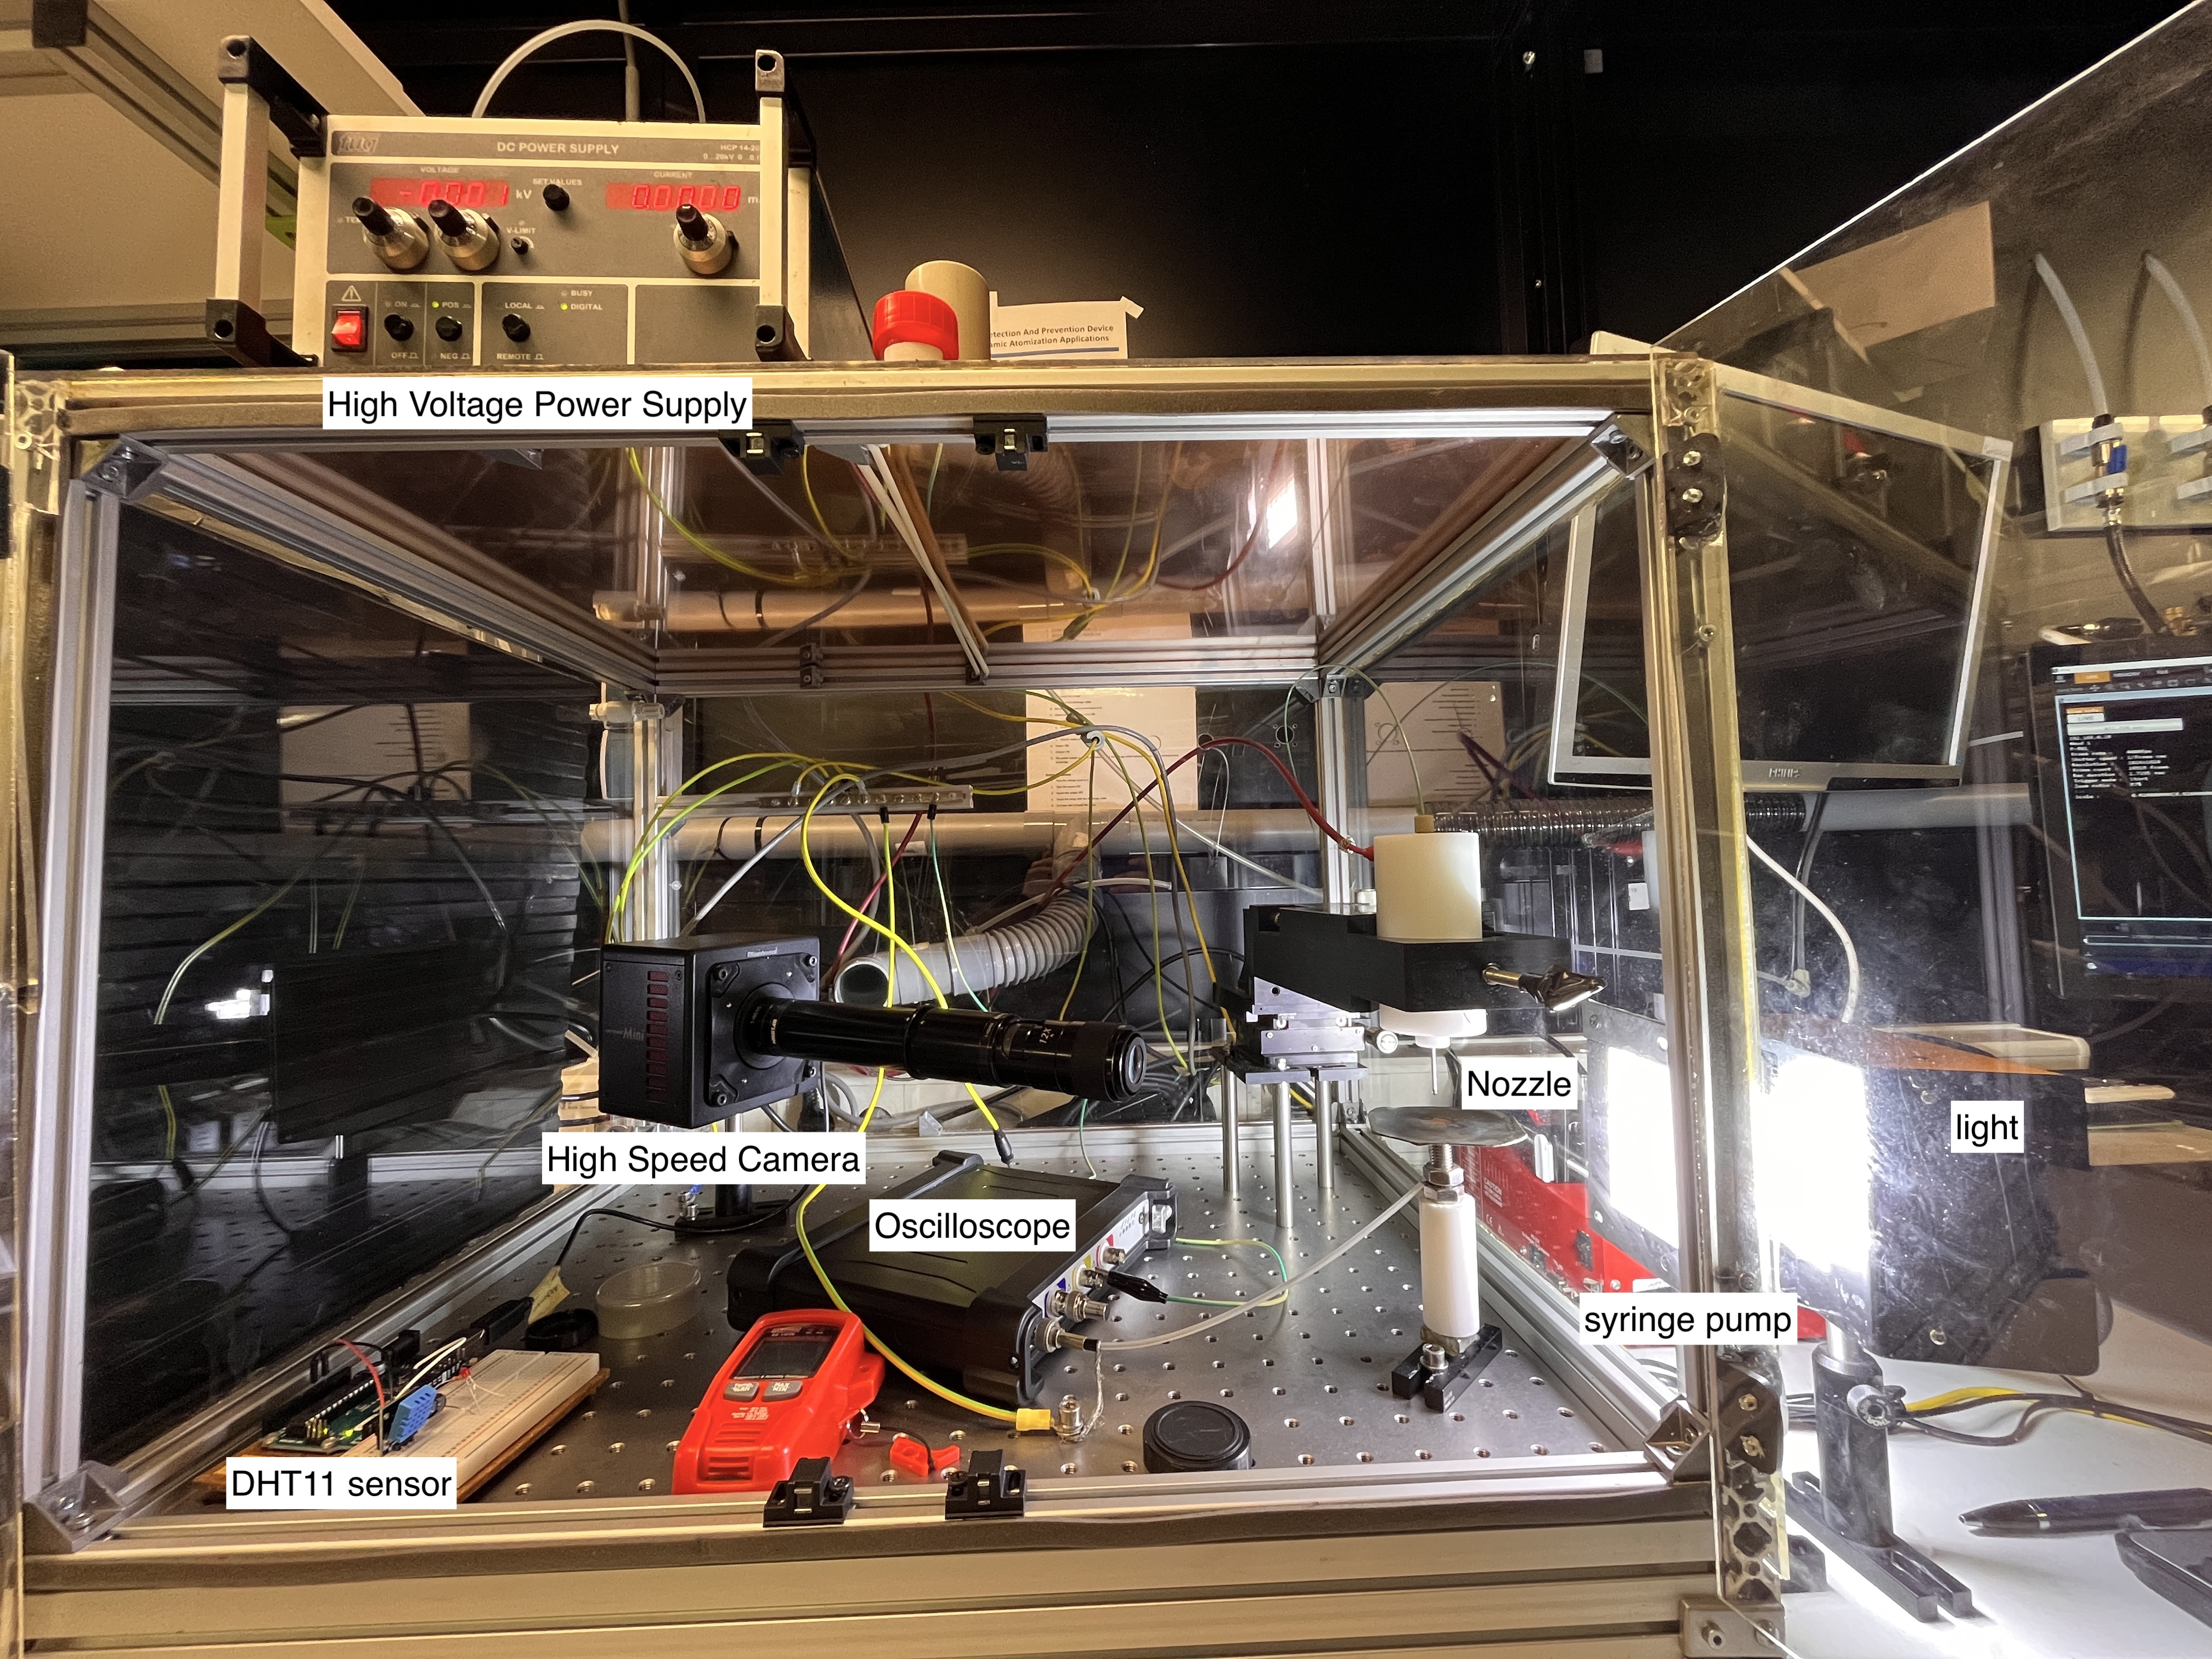
\includegraphics{Figuras/setup_pic.jpg}}
  \caption{EHDA automation system setup}
  \label{fig:setup_pic}
\end{figure}

\begin{figure}[H]
    \centering
    \resizebox{100mm}{!}{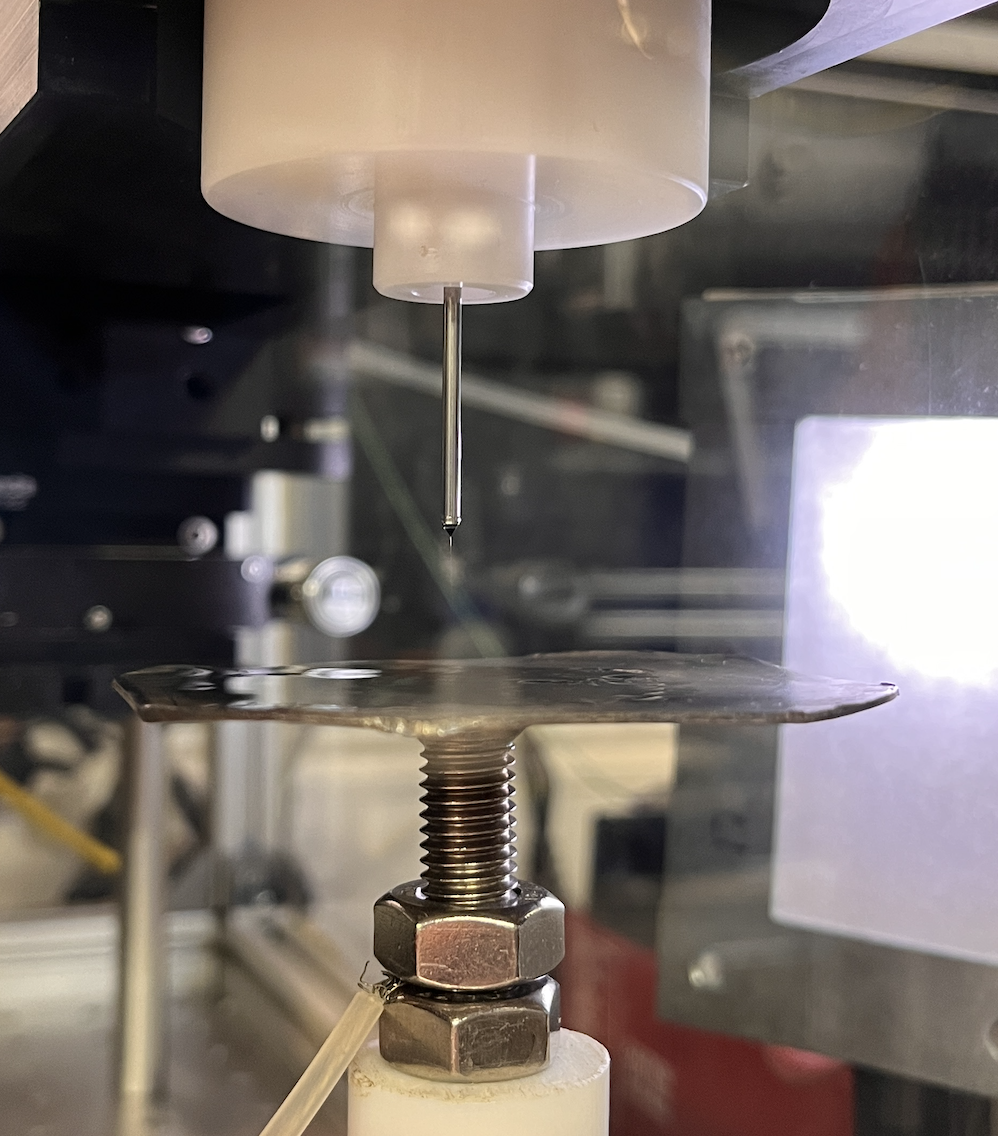
\includegraphics{Figuras/naked_eyes.png}}
    \caption{EHDA picture of the electrified syringe.}
\end{figure}







\section{Setup Validation}
\label{sec:setup_validation}


Initial tests were made to verify the setup assembly and the automation routine integration. In this step I could understand in practice how electrospray works.
It was concluded that factors like geometry, polarity, material properties and occurring discharges are reflected in the system current.
Also, liquid properties such as surface tension, dielectric constant, viscosity, density, electrical conductivity and vacuum permittivity. 
 And also physical variables such as flow rate, system impedance, system temperature, system humidity, nozzle to plate distance, nozzle dimensions and applied voltage.


 About the setup, integrate was changed the liquid, nozzle diameter and distance to the plate in order to
make the experiment the most stable and easy to reach cone-jet mode as possible. For example, while doing experiments we discovered that the frequency of the pump machine internal motors was creating an interference in the flowrate. Therefore compromising the stabilization in cone jet mode. A solution for that was to increasethe flowrate wich smooths this pumping noise. For that was also necessary to increase the nozzle diameter to balance with all other variables from the experiment.


\section{Oscilloscope Impedance}
\label{sec:osc_impedance}

The current is being measured by the Oscilloscope using its internal impedance. 
This oscilloscope model has two impedance options, 1Mohm or 2Mohms. 
Selecting one or other can multiply or divide your current measurement by 2. 
By default we are using the 2Mohm differential input. But it was noticed that using the 1Mohm resistance might reduce the noise. 
A proposal of optimization is to configure the 1Mohm resistance in the \emph{configuration\_tiepie.py} file and evaluate its performance.